% gepisat-3_nxtgn.tex
%
% written by Tyler W. Davis
% Imperial College London
%
% 2015-03-18 -- created
% 2015-03-22 -- last updated
%
% ------------
% description:
% ------------
% This TEX file contains the next-generation light-use efficiency model.
%
% ----------
% changelog:
% ----------
% 01. modularized chapter [15.03.18]
% 02. newline for each sentence [15.03.18]
% --> simpler for Git version control
% 03. added subsections [15.03.20]
% 04. added new section, testing and development [15.03.22]
%
%% \\\\\\\\\\\\\\\\\\\\\\\\\\\\\\\\\\\\\\\\\\\\\\\\\\\\\\\\\\\\\\\\\\\\\\\\ %%
%% PART 3.2 -- THE NEXT-GENERATION MODEL
%% //////////////////////////////////////////////////////////////////////// %%
\section{The Next-Generation Model}
\label{sec:nxtgen}
At the heart of GePiSaT is a production efficiency or ``diagnostic'' model for estimating monthly GPP. 
Similar to most other production efficiency models, GPP is expressed as a function of absorbed light, $I_{abs}$.
The basic equation for monthly GPP takes the form:
%% ------------------------------------------------------------------------ %%
%% eq:pem | Production efficiency model
%% ------------------------------------------------------------------------ %%
\begin{equation}
\label{eq:pem}
    \text{GPP} = \varepsilon\; I_{abs} 
\end{equation}

\noindent where:\\
\indent GPP = gross primary production [mol~C~m$^{-2}$~mo$^{-1}$];\\
\indent $I_{abs}$ = absorbed photosynthetic light; [mol~photons~m$^{-2}$~mo$^{-1}$];\\
\indent $\varepsilon$ = light-use efficiency [mol~C~mol~photons$^{-1}$].\\

\noindent The light-use efficiency, $\varepsilon$, is therefore defined as the ratio of GPP to absorbed light. 

The absorbed photosynthetic light is defined as the fraction of absorbed photosynthetically active radiation (PAR) and is calculated as the product of fPAR and PPFD (i.e., PAR in units of quanta).

Despite the simplicity of Eq. \ref{eq:pem}, this basic model performs rather well at a few of the flux tower sites. 
However, in the effort of building a universal model of terrestrial GPP, Eq. \ref{eq:pem} does not capture the global dynamics of GPP; therefore, a next-generation model is proposed based on \emph{The Coordination Hypothesis}, which states \parencite{maire12}:
\begin{quote}
	``photosynthesis is co-limited by the carboxylation and regeneration of ribulose-1,5-bisphosphate (RuBP)''
\end{quote}
where $J_\text{max}$ limitation (i.e., the light harvesting capacity) of photosynthesis is accounted by the hypothesis of an optimality between the cost and benefit of maintaining a certain light-harvesting capacity.
The theoretical model, using the empirical expression for the potential rate of electron transport by \cite{smith37}, takes the following form:
%% ------------------------------------------------------------------------ %%
%% eq:nglue | Production efficiency model
%% ------------------------------------------------------------------------ %%
\begin{equation}
\label{eq:nglue}
    \text{GPP} = \phi_{\circ}\; \text{f}_\alpha\; I_{abs}\; \sqrt{m^2 - c^{2/3}\; m^{4/3}}
\end{equation}

\noindent where:\\
\indent $\phi_{\circ}$ = intrinsic quantum efficiency [0.093~mol~C~mol~photons$^{-1}$];\\
\indent $c$ = maintenance cost of light-harvesting capacity [0.41];\\
\indent $I_{abs}$ = absorbed photosynthetic light [mol~photons~m$^{-2}$~mo$^{-1}$];\\
\indent f$_\alpha$ = index of plant available moisture;\\
\indent $m$ = substrate limitation term.\\

Equation \ref{eq:nglue} introduces two constants (i.e., $\phi_{\circ}$ and $c$) and two variables (i.e., f$_\alpha$ and $m$).
The intrinsic quantum efficiency, \nomenclature{$\phi_{\circ}$}{intrinsic quantum efficiency [0.093~mol~C~mol~photons$^{-1}$]}$\phi_{\circ}$, is assumed a constant value of 0.093 mol~C~mol~photons$^{-1}$, based on the mean of eleven measured species by \cite{long93}. 
The cost for a plant to have a certain light-harvesting capacity, \nomenclature{$c$}{maintenance cost of light-harvesting capacity [0.41]}$c$, set to a constant value 0.41, is empirically derived from reanalysis data of $J_\text{max}$ to $V_\text{cmax}$ ratios presented by \cite{kattge07}.

The index of plant available moisture, f$_\alpha$, is based on the Cramer-Prentice bioclimatic moisture index, $\alpha^\star$ (see \S \ref{sec:gepcp}). 
To maintain a coefficient that varies between 0 and 1 and to emphasize the effect of low soil moisture on limiting GPP, f$_\alpha$ is set equal to the quarter power of $\alpha^\star$ divided by its maximum value or simply: 
\nomenclature{$\text{f}_\alpha$}{index of plant available moisture}
$\text{f}_\alpha = \left(\alpha^\star/1.26\right)^{1/4}$.

The substrate limitation term, $m$, is given by:
%% ------------------------------------------------------------------------ %%
%% eq:msimp | The simplification of m
%% ------------------------------------------------------------------------ %%
\nomenclature{$m$}{substrate limitation term [unitless]}%
\begin{equation}
\label{eq:m}
    m = \frac{c_a - \Gamma^\star}
             {c_a 
              + 2 \Gamma^\star 
              + 3 \Gamma^\star \sqrt{
                1.6\; \eta^\star\; D\; \left[
                  \beta^\star\: \left(K + \Gamma^\star\right)
                \right]^{-1}
              }
             }
\end{equation}

\noindent where:\\
\indent $\beta^\star$ = standardized cost ratio [244.0];\\
\indent $\eta^\star$ = relative viscosity of water [unitless];\\
\indent $c_a$ = partial pressure of atmospheric CO$_2$ [Pa];\\
\indent $D$ = vapor pressure deficit [Pa];\\
\indent $\Gamma^\star$ = photorespiratory compensation point [Pa];\\
\indent $K$ = Michaelis-Menten rubisco-limited photosynthesis coefficient [Pa].\\

\noindent The following subsections discuss each of the variables used in the calculation of $m$.

%% \\\\\\\\\\\\\\\\\\\\\\\\\\\\\\\\\\\\\\\\\\\\\\\\\\\\\\\\\\\\\\\\\\\\\\\\ %%
%% PART 3.2.1 -- THE STANDARDIZED COST RATIO
%% //////////////////////////////////////////////////////////////////////// %%
\subsection{The Standardized Cost Ratio}
\label{sec:beta}
\nomenclature{$\beta^\star$}{standardized cost ratio [244.0]}%
The semi-empirical constant, $\beta^\star$, reflects the ratio of the cost factors for carboxylation and transpiration at standard temperature (i.e., 25 ${}^\circ$C) and sea level. 
The derivation of $\beta^\star$ is based on \emph{The Least-Cost Hypothesis}, which states \parencite{prentice14}:
\begin{quote}
	''plant leaves minimize the summed unit costs of transpiration and carboxylation.''
\end{quote}
To begin, we introduce $\chi$ as the ratio between leaf internal, $c_i$, and ambient, $c_a$, mole fractions of CO$_2$, which is known to decline with vapor pressure deficit, $D$, in the following form:
%% ---------------------------------------------------------------%%
%% eq:chi | Chi
%% ---------------------------------------------------------------%%
\begin{equation}
\nomenclature{$\chi$}{ratio of leaf internal to ambient mole fraction of CO$_2$ [unitless]}%
\label{eq:chi}
    \chi = \frac{\xi}{\xi + \sqrt{D}}
\end{equation}

\noindent where $\xi$ is carbon cost of water, which may be simply expressed by:
%% ---------------------------------------------------------------%%
%% eq:xi | Xi
%% ---------------------------------------------------------------%%
\nomenclature{$\xi$}{carbon cost of water [unitless]}%
\begin{equation}
\label{eq:xi}
    \xi = \sqrt{\frac{K\; b}{1.6\; a}} = \sqrt{\frac{K\; \beta^\star}{1.6\; \eta^\star}}
\end{equation}

\noindent where:\\
\indent $a$ = carbon cost of maintaining transpiration for assimilation; \\
\indent $b$ = cost of maintaining photosynthetic proteins for assimilation;\\
\indent $K$ = Michaelis-Menten rubisco-limited photosynthesis coefficient [Pa];\\
\indent $\eta^\star$ = relative viscosity of water.\\

Based on Eq. \ref{eq:xi}, $\beta^\star$ is equal to $\eta^\star\: b/a$.
Taking the inverse logistic sigmoidal function of $\chi$, substituting the definition of $\xi$ from Eq. \ref{eq:xi} into Eq. \ref{eq:chi}, the temperature and elevation effects of $D$, $K$, and $\eta^\star$ on $\chi$ may be explicitly expressed (via partial differentiation):
%% ---------------------------------------------------------------%%
%% eq:whe | Wang Han equation
%% ---------------------------------------------------------------%%
\begin{equation}
\label{eq:whe}
    \ln \left(\frac{\chi_o}{1 - \chi_o}\right) = 4.64 + 
    	0.0545\: \left(T_{air} - 25\right) - 
    	0.5\; \ln (D) - 
    	8.15\times 10^{-5}\; z
\end{equation}

\noindent where:\\
\indent $T_{air}$ = air temperature [${}^\circ$C];\\
\indent $D$ = vapor pressure deficit [Pa];\\
\indent $\chi_o$ = optimal value of $\chi$ [unitless];\\
\indent $z$ = altitude above mean sea level [m].\\

\noindent At mean sea level (i.e., $z = 0$), standard temperature (i.e., $T_{air} = 25\;{}^\circ$C), and an ideal vapor pressure deficit (i.e., $D = 1000$ Pa), the optimal value of $\chi$ is 0.767. Substituting this value of $\chi$ and the expression of $\xi$, given in Eq. \ref{eq:xi} (where $K = 70.84$ Pa at 25 ${}^\circ$C), into Eq. \ref{eq:chi}, $\beta^\star$ is found to be 244.0. 

%% \\\\\\\\\\\\\\\\\\\\\\\\\\\\\\\\\\\\\\\\\\\\\\\\\\\\\\\\\\\\\\\\\\\\\\\\ %%
%% PART 3.2.2 -- RELATIVE VISCOSITY OF WATER
%% //////////////////////////////////////////////////////////////////////// %%
\subsection{Relative Viscosity of Water}
\label{sec:eta}
The viscosity of water at a given temperature and pressure, $\eta$, may be calculated based on the methodology of \cite{huber09}. 
The relative viscosity of water with respect to its value at 25 ${}^\circ$C, $\eta^\star$, is calculated by the following ratio:
%% ---------------------------------------------------------------%%
%% eq:ns | Relative viscosity of water
%% ---------------------------------------------------------------%%
\nomenclature{$\eta^\star$}{relative viscosity of water [unitless]}%
\begin{equation}
\label{eq:ns}
    \eta^\star = \frac{\eta}{\eta_{25}}
\end{equation}

\noindent where:\\
\indent $\eta$ = viscosity of water at a given temperature and pressure [Pa s];\\
\indent $\eta_{25}$ = viscosity at 25 ${}^\circ$C and standard pressure [8.90$\times 10^{-4}$ Pa s].\\

%% \\\\\\\\\\\\\\\\\\\\\\\\\\\\\\\\\\\\\\\\\\\\\\\\\\\\\\\\\\\\\\\\\\\\\\\\ %%
%% PART 3.2.3 -- AMBIENT PARTIAL PRESSURE OF CO2
%% //////////////////////////////////////////////////////////////////////// %%
\subsection{Ambient Partial Pressure of CO$_2$}
\label{sec:ca}
The partial pressure of CO$_2$, $c_a$, is calculated based on the observed annual atmospheric CO$_2$ concentration (see \S \ref{sec:gepnoaa}). 
The conversion can be done knowing the total atmospheric pressure, $P_{atm}$, and using Dalton's Law of Partial Pressure:
%% ---------------------------------------------------------------%%
%% eq:pp | Partial Pressure Convertion
%% ---------------------------------------------------------------%%
\begin{equation}
\label{eq:pp}
    p_x = 1\times 10^{-6}\; ppm_x\; P_{atm}
\end{equation}

\noindent where:\\
\indent $p_x$ = partial pressure of gas \textit{x} [Pa];\\
\indent $ppm_x$ = parts-per-million concentration of gas \textit{x} [ppm];\\
\indent $P_{atm}$ = total atmospheric pressure [Pa].\\

\noindent For instances when $P_{atm}$ is unknown, the elevation-dependent atmospheric pressure may be computed using the Barometric Formula \parencite{allen98}:
%% ---------------------------------------------------------------%%
%% eq:pz | Atmospheric pressure as a function of elevation
%% ---------------------------------------------------------------%%
\nomenclature{$P_{atm}$}{total atmospheric pressure [Pa]}%
\begin{equation}
\label{eq:pz}
    P_{atm}\left( z \right) = P_{\circ} \left( 
    	1 - \frac{L\; z}{T_{\circ}} 
    \right)^{\frac{g\; M_a}{R_u\; L}}
\end{equation}

\noindent where:\\
\indent $z$ = altitude above mean sea level [m];\\
\indent $g$ = standard gravity [9.80665 m s$^{-2}$];\\
\indent $P_{\circ}$ = base atmospheric pressure [101325 Pa];\\
\indent $L$ = temperature lapse rate [0.0065 K m$^{-2}$];\\
\indent $T_{\circ}$ = base temperature [298.15 K];\\
\indent $M_a$ = molecular weight for dry air [0.028963 kg mol$^{-1}$];\\
\indent $R_u$ = universal gas constant [8.3145 J mol$^{-1}$ K$^{-1}$].\\

%% \\\\\\\\\\\\\\\\\\\\\\\\\\\\\\\\\\\\\\\\\\\\\\\\\\\\\\\\\\\\\\\\\\\\\\\\ %%
%% PART 3.2.4 -- VAPOR PRESSURE DEFICIT
%% //////////////////////////////////////////////////////////////////////// %%
\subsection{Vapor Pressure Deficit}
\label{sec:d}
The vapor pressure deficit, $D$, is based on the unit conversion of the observed VPD (see \S \ref{sec:gepvpd}) from kPa to Pa.

%% \\\\\\\\\\\\\\\\\\\\\\\\\\\\\\\\\\\\\\\\\\\\\\\\\\\\\\\\\\\\\\\\\\\\\\\\ %%
%% PART 3.2.5 -- PHOTORESPIRATORY COMPENSATION POINT
%% //////////////////////////////////////////////////////////////////////// %%
\subsection{Photorespiratory Compensation Point}
\label{sec:gs}
\nomenclature{$\Gamma^\star$}{photorespiratory compensation point [Pa]}%
The photorespiratory compensation point, $\Gamma^\star$, depends on both the atmospheric pressure and temperature.
\cite{bernacchi01} provides the definitive equation for $\Gamma^\star$:
%% ---------------------------------------------------------------%%
%% eq:gsbasic | Basic equation of Gamma*
%% ---------------------------------------------------------------%%
\begin{equation}
\label{eq:gsbasic}
    \Gamma^\star = \frac{O\: K_c\: V_\text{o,max}}
                        {2\: K_o\: V_\text{c,max}}
\end{equation}

\noindent where:\\
\indent $O$ = partial pressure of atmospheric O$_2$, [Pa];\\
\indent $K_c$ = Michaelis-Menten constant for carboxylation [Pa];\\
\indent $K_o$ = Michaelis-Menten constant for oxygenation [Pa];\\
\indent $V_\text{c,max}$ = maximum rate of carboxylation [$\mu$mol~m$^{-2}$~s$^{-1}$];\\
\indent $V_\text{o,max}$ = maximum rate of oxygenation [$\mu$mol~m$^{-2}$~s$^{-1}$].\\

\noindent The temperature-dependency of $\Gamma^\star$ is derived from the temperature dependencies of $K_c$, $K_o$, $V_\text{c,max}$, and $V_\text{o,max}$, which have been empirically solved by \cite{bernacchi01}. 
Substituting the temperature-dependency equations for each term in Eq. \ref{eq:gsbasic}, results in the following expression:
%% ---------------------------------------------------------------%%
%% eq:gst | Temperature dependency of Gamma*
%% ---------------------------------------------------------------%%
\begin{equation}
\label{eq:gst}
    \Gamma^\star = \exp \left(7.472 - \frac{\Delta H_a}{R_u\: T_k}\right) \frac{O}{2}
\end{equation}

\noindent where:\\
\indent $\Delta H_a$ = activation energy for $\Gamma^\star$ [37$\,$830 J mol$^{-1}$];\\
\indent $R_u$ = universal gas constant [8.3145 J mol$^{-1}$ K$^{-1}$];\\
\indent $O$ = partial pressure of atmospheric O$_2$, [Pa];\\
\indent $T_k$ = leaf temperature [K].\\

\noindent To account for changes in the atmospheric pressure, the partial pressure of O$_2$ may be expressed in terms of molar fraction based on Dalton's Law (see Eq. \ref{eq:pp}):
%% ---------------------------------------------------------------%%
%% eq:gstpa | Temperature & pressure dependency of Gamma*
%% ---------------------------------------------------------------%%
\begin{equation}
\label{eq:gstpa}
    \Gamma^\star = 5\times 10^{-7}\: ppm_{O_2}\: P_{atm}\: \exp \left(7.472 - \frac{\Delta H_a}{R_u\: T_k}\right)
\end{equation}

\noindent where $ppm_{O_2}$ is the molar fraction of atmospheric O$_2$. Assuming a constant value for $ppm_{O_2}$ (i.e., 209476 ppm), $\Gamma^\star$ may be simplified to:
%% ---------------------------------------------------------------%%
%% eq:gstpb | Temperature & pressure dependency of Gamma*
%% ---------------------------------------------------------------%%
\begin{equation}
\label{eq:gstpb}
    \Gamma^\star = \exp \left(5.216 - \frac{\Delta H_a}{R_u\: T_k}\right)\: P_{atm}
\end{equation}

\noindent where:\\
\indent $\Delta H_a$ = activation energy for $\Gamma^\star$ [37$\,$830 J mol$^{-1}$];\\
\indent $R_u$ = universal gas constant [8.3145 J mol$^{-1}$ K$^{-1}$];\\
\indent $P_{atm}$ = atmospheric pressure [Pa];\\
\indent $T_k$ = leaf temperature [K].\\

\noindent Due to a general lack of understanding, the leaf temperature in Eq. \ref{eq:gst}, $T_k$, may be substituted by the ambient air temperature, $T_{air}$, in units of Kelvin. 

%% \\\\\\\\\\\\\\\\\\\\\\\\\\\\\\\\\\\\\\\\\\\\\\\\\\\\\\\\\\\\\\\\\\\\\\\\ %%
%% PART 3.2.6 -- MICHAELIS-MENTON COEFFICIENT
%% //////////////////////////////////////////////////////////////////////// %%
\subsection{Michaelis-Menten Coefficient of Photosynthesis}
\label{sec:k}
\nomenclature{$K$}{Michaelis-Menten coefficient of photosynthesis [Pa]}%
The Michaelis-Menten coefficient of Rubisco-limited photosynthesis is a function of the Rubisco photosynthetic rates for O$_2$ and CO$_2$ \parencite{farquhar80}:
%% ------------------------------------------------------------------------ %%
%% eq:michaelis | Michaelis Menten coefficient
%% ------------------------------------------------------------------------ %%
\begin{equation}
\label{eq:michaelis}
	K = K_c\: \left( 1 + \frac{O}{K_o} \right)
\end{equation}

\noindent where:\\
\indent $K_c$ = Michaelis-Menten constant for CO$_2$ [Pa];\\
\indent $K_o$ = Michaelis-Menten constant for O$_2$ [Pa];\\
\indent $O$ = partial pressure of atmospheric O$_2$, [Pa].\\

\noindent The Michaelis-Menton constants for CO$_2$ and O$_2$ ($K_c$ and $K_o$, respectively) have temperature dependencies, which have been empirically fit to the Arrhenius function and normalized to 25~$^\circ$C \parencite{farquhar80}:
%% ------------------------------------------------------------------------ %%
%% eq:kcko | Michaelis Menten Kc & Ko coefficients
%% ------------------------------------------------------------------------ %%
\nomenclature{$K_c$}{Michaelis-Menten constant for CO$_2$ [Pa]}%
\nomenclature{$K_o$}{Michaelis-Menten constant for O$_2$ [Pa]}%
\begin{subequations}
\label{eq:kcko}
\begin{align}
	K_c&=K_{c25}\: \exp \left[ 
    	\frac{\Delta H_{a,c}\: \left(T_k-298.15\right)}{298.15\: R_{u}\: T_k}
    \right] \label{eq:kc} \\
    K_o&=K_{o25}\: \exp \left[ 
    	\frac{\Delta H_{a,o}\: \left(T_k-298.15\right)}{298.15\: R_{u}\: T_k}
    \right] \label{eq:ko}
\end{align}
\end{subequations}

\noindent where:\\
\indent $K_{c25}$ = Michaelis-Menten constant for CO$_2$ at 25~$^{\circ}$C [Pa];\\
\indent $K_{o25}$ = Michaelis-Menten constant for O$_2$ at 25~$^{\circ}$C [Pa];\\
\indent $\Delta H_{a,c}$ = activation energy for carboxylation [79$\,$430 J mol$^{-1}$];\\
\indent $\Delta H_{a,o}$ = activation energy for oxygenation [36$\,$380 J mol$^{-1}$];\\
\indent $R_{u}$ = universal gas constant [8.3145 J mol$^{-1}$ K$^{-1}$];\\
\indent $T_k$ = leaf temperature [K].\\

\noindent Once again, leaf temperature, as in Eqns. \ref{eq:michaelis} and \ref{eq:kcko}, may be substituted by the ambient air temperature, $T_{air}$, converted to units of Kelvin. 

The partial pressure values of $K_{c25}$ and $K_{o25}$ are based on the empirical temperature dependencies given by \cite{bernacchi01}, in mole fractions, converted to partial pressures by Dalton's Law (see Eq. \ref{eq:pp}):
%% ------------------------------------------------------------------------ %%
%% eq:kcko25 | Michaelis Menten Kc & Ko coefficients
%% ------------------------------------------------------------------------ %%
\nomenclature{$K_{c25}$}{Michaelis-Menten coefficient of carboxylation at 25~$^\circ$C [Pa]}%
\nomenclature{$K_{o25}$}{Michaelis-Menten coefficient of oxygenation at 25~$^\circ$C [Pa]}%
\begin{subequations}
\label{eq:kcko25}
\begin{align}
	K_{c25}&=1\times 10^{-6} \exp \left[ 38.05 - 
    	\frac{\Delta H_{a,c}}{298.15\: R_{u}}
    \right]\: P_{atm} \label{eq:kc25} \\
    K_{o25}&=1\times 10^{-3} \exp \left[ 20.30 - 
    	\frac{\Delta H_{a,o}}{298.15\: R_{u}}
    \right]\: P_{atm} \label{eq:ko25}
\end{align}
\end{subequations}

\noindent Assuming that the experiments conducted at the University of Illinois at Urbana-Champaign were performed under atmospheric pressure (at elevation 227 m above mean sea level), the partial pressure of $K_{c25}$ is 39.97 Pa and the partial pressure of $K_{o25}$ is 27$\,$480 Pa and are invariant to changes in atmospheric pressure.

%% \\\\\\\\\\\\\\\\\\\\\\\\\\\\\\\\\\\\\\\\\\\\\\\\\\\\\\\\\\\\\\\\\\\\\\\\ %%
%% PART 3.3 -- MODEL TESTING AND DEVELOPMENT
%% //////////////////////////////////////////////////////////////////////// %%
\section{Model Testing and Development}
\label{sec:modeldev}
The next-generation model described in \S \ref{sec:nxtgen} was developed under the constraints of in-situ observations and measurements. 
To test the model, a open-source framework was established consisting of two parts.
The first is a PostgreSQL database, which stores the various observations for unified data access (see Part \ref{partii} for details).
The second is the Python application code, which integrates with the database, written to be easily readable and reproducible while still being computationally powerful (see Part \ref{parti} for more details).

The key inputs required for model testing and comparison include in-situ measurements of half-hourly net ecosystem exchange and photosynthetic flux density (\S \ref{sec:gepfluxd}) and annual atmospheric CO$_2$ concentration (\S \ref{sec:gepnoaa}) along with remotely sensed gridded observations of daily shortwave solar radiation (\S \ref{sec:gepwatch}), monthly vegetative greenness (\S \ref{sec:gepmodis}), and various monthly meteorological observations (\S \ref{sec:gepvpd} and \ref{sec:gepcru}).

%% \\\\\\\\\\\\\\\\\\\\\\\\\\\\\\\\\\\\\\\\\\\\\\\\\\\\\\\\\\\\\\\\\\\\\\\\ %%
%% PART 3.4 -- FLUX PARTITIONING
%% //////////////////////////////////////////////////////////////////////// %%
\section{Flux Partitioning}
\label{sec:fluxparti}
The first step in the model testing is to derive the monthly observed GPP from the flux tower measurements.
As GPP is not observed at the flux towers, it is therefore necessary to empirically decompose the high resolution CO$_{2}$ flux into quantities of GPP and ecosystem respiration (R$_{\mathrm{e}}$) based on the theoretical expression for net ecosytem exchange (NEE) \parencite{lovett06}:
%% ------------------------------------------------------------------------ %%
%% eq:nee | Net ecosystem exchange
%% ------------------------------------------------------------------------ %%
\nomenclature{$\text{NEE}$}{net ecosystem exchange [$\mu$mol CO$_2$ m$^{-2}$ s$^{-1}$]}%
\begin{equation}
\label{eq:nee}
    \text{NEE} = \text{R}_{\text{e}} - \text{GPP}
\end{equation}

\noindent where:\\
\indent NEE = net ecosystem exchange [$\mu$mol CO$_2$ m$^{-2}$ s$^{-1}$];\\
\indent R$_\text{e}$ = ecosystem respiration [$\mu$mol CO$_2$ m$^{-2}$ s$^{-1}$];\\
\indent GPP = gross primary production [$\mu$mol CO$_2$ m$^{-2}$ s$^{-1}$].\\

\noindent The convention presented in equation \ref{eq:nee} indicates that positive CO$_{2}$ exchange occurs in the form of ecosystem respiration (i.e., adding CO$_{2}$ into the atmosphere) and negative exchange occurs during photosynthesis (i.e., atmospheric carbon sequestration into plant leaves). 

There are several models that combine leaf photosynthesis (e.g., GPP) and radiation transfer (e.g., PPFD) through a vegetated canopy.  
In \parencite{ruimy95}, the response curve of leaves to radiative energy is assumed to follow one of two models described below (rearranged for consistency with the sign convention presented in Eq. \ref{eq:nee}).  
Equation \ref{eq:modell} represents the ``linear'' response model and Eq. \ref{eq:modelh} represents the ``rectangular hyperbola'' response model.
%% ------------------------------------------------------------------------ %%
%% eq:fmodels | GPP partitioning (Ruimy's models)
%% ------------------------------------------------------------------------ %%
\begin{subequations}
\label{eq:fmodels}
\begin{align}
    F &= R - \alpha\: Q \label{eq:modell} \\
    F &= R - \frac{\alpha\: F_\infty\: Q}
                  {\alpha\: Q + F_\infty}\label{eq:modelh}
\end{align}
\end{subequations}

\noindent where:\\
\indent $F$ = CO$_2$ exchange rate [$\mu$mol CO$_2$ m$^{-2}$ s$^{-1}$];\\
\indent $R$ = dark respiration rate [$\mu$mol CO$_2$ m$^{-2}$ s$^{-1}$];\\
\indent $Q$ = quantum flux density (e.g., PPFD) [$\mu$mol photons m$^{-2}$ s$^{-1}$];\\
\indent $\alpha$ = apparent quantum yield (i.e., d$F$/d$Q$ at $Q=0$);\\
\indent $F_{\infty}$ = $F$ at saturating quantum yield [$\mu$mol CO$_2$ m$^{-2}$ s$^{-1}$].\\

By combining Eqns. \ref{eq:fmodels} with Eq. \ref{eq:nee}, GPP partitioning can be obtained, setting $\text{NEE} = F$ and $\text{R}_{\text{e}} = R$, through least squares regression in the following forms:
%% ------------------------------------------------------------------------ %%
%% eq:neemodels | NEE models (Ruimy's models)
%% ------------------------------------------------------------------------ %%
\begin{subequations}
\label{eq:neemodels}
\begin{align}
    \text{NEE} &= R - \alpha\; (\text{PPFD}) \label{eq:linmod}\\
    \text{NEE} &= \frac{a\; (\text{PPFD}) + b}
                       {c\; (\text{PPFD}) + d}\label{eq:hypmod}
\end{align}
\end{subequations}

\noindent where:
%% ------------------------------------------------------------------------ %%
%% eq:shyp | Hyperbolic model definition of parameters
%% ------------------------------------------------------------------------ %%
\begin{subequations}
\label{eq:shyp}
\begin{align}
    a&= \alpha\: R - \alpha\: F_{\infty} \label{eq:shypa}\\
    b&= F_{\infty}\: R \label{eq:shypb}\\
    c&= \alpha \label{eq:shypc}\\
    d&= F_{\infty} \label{eq:shypd}
\end{align}
\end{subequations}

\noindent Note that the form of the rectangular hyperbola presented in Eq. \ref{eq:hypmod} has an x-axis asymptote defined by $a/c$ from Eqns. \ref{eq:shypa} and \ref{eq:shypc}. 


%%
%% Add outlier removal
%%
%% \\\\\\\\\\\\\\\\\\\\\\\\\\\\\\\\\\\\\\\\\\\\\\\\\\\\\\\\\\\\\\\\\\\\\\\\ %%
%% PART 3.4.1 -- OUTLIER REMOVAL
%% //////////////////////////////////////////////////////////////////////// %%
\subsection{Outlier removal}
\label{sec:mst1out}
While there are morality debates over whether outliers should be removed at all from observation datasets, it is well known that outliers are detrimental when present during model fitting.  
This project is trying to address large scale processes and therefore removing outliers from instantaneous measurement fields to improve the fitted relationships between NEE and PPFD is viewed as acceptable.

To provide a robust and statistically-based approach for identifying outliers for the data pairs of NEE and PPFD, Peirce's criterion is used \parencite{peirce52}.  
The main issue revolving around Peirce's criterion is the calculation of the maximum allowable deviation of a measurement (i.e., the threshold error).  
To help facilitate this difficulty, tables of values were developed and published by B.A. Gould, Jr. \parencite{gould55}.  
Unfortunately, flux tower datasets often have numbers of observations that far exceed the values provided in Gould's tables. 
Therefore, in order to use Peirce's criterion, the error threshold values must be calculated.

The methodology follows Gould's algorithm and the calculation utilizes a Newtonian-style convergence method as presented by K. Thomsen\footnotemark. \footnotetext{http://mathforum.org/kb/thread.jspa?forumID=13\&threadID=1841790\\ \indent\&messageID=6449606} 
The principle of Peirce's criterion for identifying outliers is that \parencite{peirce52}:
\begin{quote}
``the proposed observations should be rejected when the probability of the system of errors obtained by retaining them is less than that of the system of errors obtained by their rejection multiplied by the probability of making so many, and no more, abnormal observations.''
\end{quote}

In this principle, Peirce proposes two systems, one where outliers have been identified and removed and the original system.  
To express this idea, the following condition for rejection is made \parencite[Eq. A]{gould55}:
%% ------------------------------------------------------------------------ %%
%% eq:goulda | Gould's equation A
%% ------------------------------------------------------------------------ %%
\begin{equation}
\label{eq:goulda}
    \lambda^{N-n}\; e^{0.5\: n\: (x^{2}-1)}\; \left(\psi\: x\right)^{n} < Q_{pc}^{N}
\end{equation}

\noindent where: \\
\indent $\lambda$ = ratio of mean errors between the two systems;\\
\indent $N$ = number of observations;\\
\indent $n$ = number of outliers;\\
\indent $x$ = residual error;\\
\indent $\psi\: x$ = probability of error exceedance (hyperbolic base);\\
\indent $Q_{pc}$ = represents the condition for rejection.\\ 

\noindent $Q_{pc}$ is given by \parencite[Eq. B]{gould55}:
%% ------------------------------------------------------------------------ %%
%% eq:gouldb | Gould's equation B
%% ------------------------------------------------------------------------ %%
\begin{equation}
\label{eq:gouldb}
    Q_{pc}^{N} = \frac{n^{n}\;(N-n)^{N-n}}{N^{N}}
\end{equation}

Peirce proposes to begin with the assumption that the excess in the sum of the squared errors from the original system (compared to the system where outliers are removed) is equal to the sum of the squared errors of the outliers.  
This presents the following equation \parencite[Eq. C]{gould55}:
%% ------------------------------------------------------------------------ %%
%% eq:gouldc | Gould's equation C
%% ------------------------------------------------------------------------ %%
\begin{equation}
\label{eq:gouldc}
    x^{2} = 1 + \frac{N-m-n}{n}\; \left(1 - \lambda^{2}\right)
\end{equation}

\noindent where: \\
\indent $x^{2}$ = Peirce's deviation (squared error threshold) \\
\indent $m$ = number of unknowns (fitting parameters) in the system \\

To solve this system of equations (i.e., determine the critical error, $x^{2}$, for which observations with a squared error less than this value should be kept and observations with a squared error greater than this value should be rejected), an iterative approach can be made by first allowing the following equality \parencite[Eq. D]{gould55}:
%% ------------------------------------------------------------------------ %%
%% eq:gouldd | Gould's equation D
%% ------------------------------------------------------------------------ %%
\begin{equation}
\label{eq:gouldd}
    R_{pc} = e^{0.5\:(x^2-1)}\; \psi\: x
\end{equation}

\noindent to be substituted into equation \ref{eq:goulda} to obtain the following \parencite[Eq. A$'$]{gould55}:
%% ------------------------------------------------------------------------ %%
%% eq:gouldap | Gould's equation A'
%% ------------------------------------------------------------------------ %%
\begin{equation}
\label{eq:gouldap}
    \lambda^{N-n}\; R_{pc}^{n} = Q_{pc}^{N}
\end{equation}

\noindent Now, for a given number of observations (i.e., $N$), an assumed number of outliers (i.e., $n$), and the number of fitting parameters used in the regression (i.e., $m$), the critical observation residual error (i.e., $x$) for identifying outliers can be calculated as follows:

\begin{enumerate}
    \item Calculate $Q_{pc}$ based on the N$^{th}$ root (equation \ref{eq:gouldb})
    \item Assume a starting value for $R_{pc}$ (e.g., 1.0)
    \item Calculate $\lambda$ based on the current $R$ value by taking the 
          1/(N-n)$^{th}$ root (equation \ref{eq:gouldap})
    \item Calculate $x^{2}$ based on the current $\lambda$ value (equation
          \ref{eq:gouldc})
    \item Calculate $R_{pc}$ based on the current $x^{2}$ value (equation 
          \ref{eq:gouldd})
    \item Compare the new $R_{pc}$ value to the one in step 3
    \item Repeat steps 3--6 until the difference between $R_{pc}$ values is 
          negligible 
\end{enumerate}

\noindent This algorithm can be expressed in the Python programming language by taking advantage of the third party modules NumPy\footnotemark \footnotetext{\url{http://www.numpy.org}} and SciPy\footnotemark. \footnotetext{\url{http://www.scipy.org}} 
An example of the code is given in Appendix \ref{app:peircepy}.

The following algorithm (example available in Appendix \ref{app:outlierpy}) can be used to make use of this code in identifying outliers in the GPP partitioning: 

\begin{enumerate}
    \item Fit a model (e.g., equation \ref{eq:linmod} or \ref{eq:hypmod}) to
          the observation data (i.e., NEE and PPFD pairs)
    \item Calculate the model's squared residual errors:\\
          %% ---------------------------------------------------------------%%
          %% eq:residerr | Residual error calculation
          %% ---------------------------------------------------------------%%
          \begin{equation}
          \label{eq:residerr}
              x_{i}^{2} = \left(U_{i}-u_{i}\right)^{2}
          \end{equation}
          where: $U_{i}$ = $i^{th}$ observation and $u_{i}$ = $i^{th}$ model 
          prediction
    \item Calculate the model mean squared error (MSE):\\
          %% ---------------------------------------------------------------%%
          %% eq:mse | Mean-squared error calculation
          %% ---------------------------------------------------------------%%
          \begin{equation}
          \label{eq:mse}
              \text{MSE} = \frac{\sum_{i=1}^{N}\left(U_{i}-u_{i}\right)^{2}}
                                {N-m}
          \end{equation}
          where: $N$ is the number of observations and $m$ is the number of 
          regressors (i.e., model coefficients)
    \item Assume one outlier exists in the observation pairs (i.e., $n=1$)
    \item Calculate Peirce's $x^{2}$ using the Python script
    \item Calculate the maximum squared error deviation:\\
          %% ---------------------------------------------------------------%%
          %% eq:delta2 | Squared deviation (delta) calculation
          %% ---------------------------------------------------------------%%
          \begin{equation}
          \label{eq:delta2}
              \Delta^{2} = \text{MSE}\; x^{2}
          \end{equation}
    \item Identify any squared errors, $x_{i}^{2}$ (from step 2), greater than 
          $\Delta^{2}$
    \item Increment $n$ and repeat steps 5--7 until the number of outliers 
          found is less than $n$
\end{enumerate}

%% ------------------------------------------------------------------------ %%
%% fig:outlier | Peirce's criterion outlier identification/removal (red)
%% ------------------------------------------------------------------------ %%
\begin{figure}[h!]
    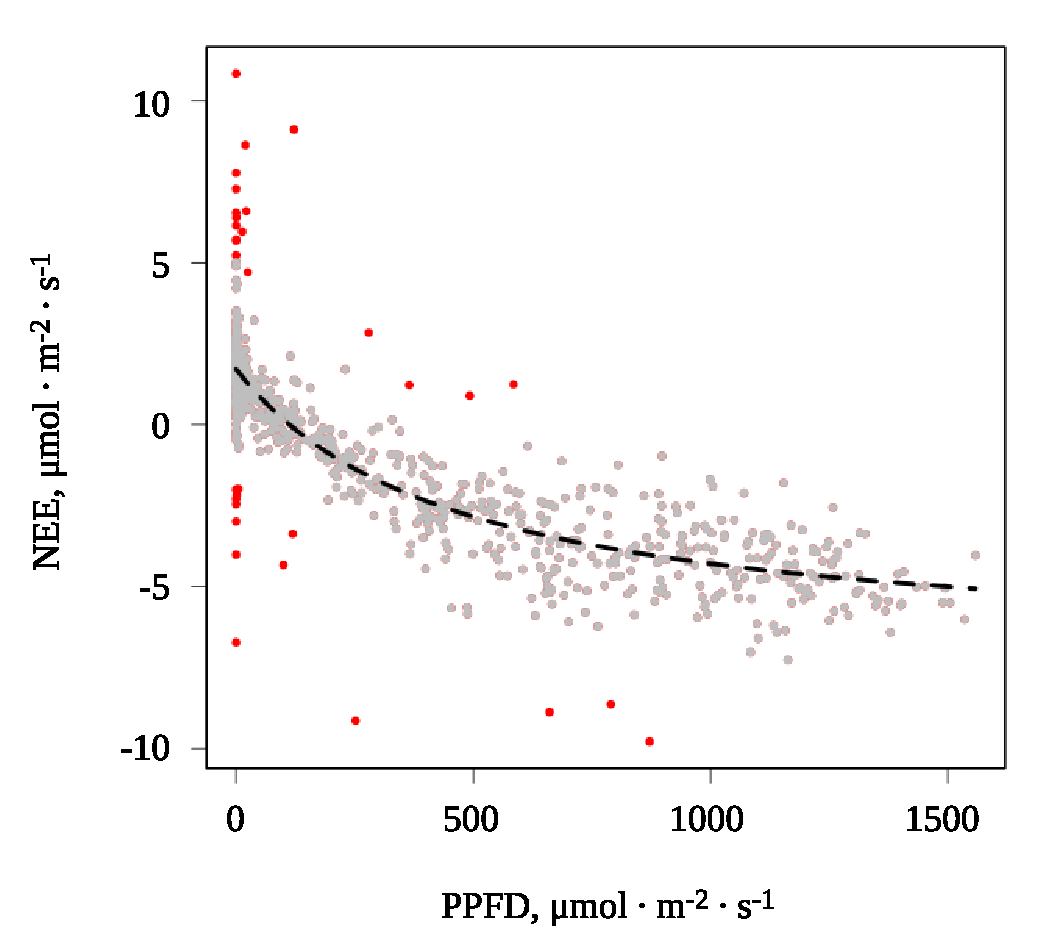
\includegraphics[width=0.85\textwidth]{olr_sedeg.eps}
    \caption{Plot of PPFD versus NEE for the month of August, 2004 for flux 
    tower SE-Deg (Sweden). Data points highlighted in red represent outliers 
    removed using the Peirce criterion. The dashed line represents the flux 
    partitioning as fitted by equation \ref{eq:hypmod}: $\alpha = 0.0189$, 
    $F_{\infty} = 8.8$, $R = 1.72$. The model fit coefficient of determination, 
    $R^{2}$, is 0.757 before outliers are removed and 0.872 after removal.}
    \label{fig:outlier}
\end{figure}

\noindent Figure \ref{fig:outlier} shows an example of the GPP partitioning for flux tower SE-Deg (located in Sweden) during May of 2002.  
Outliers identified by the Peirce criterion are highlighted in red ($N_{outliers} = 14$).  
Peirce's criterion successfully identifies observation pairs distant from the optimization curve (dashed line).  
Following the removal of the outliers, the partitioning regression fitness (based on equation \ref{eq:hypmod}) improves ($R^{2} = 0.796$ for the original observations; $R^{2} = 0.884$ after outliers are removed).  
In most cases, outliers are identified in a manner similar to that presented in Figure \ref{fig:outlier}.  
However, some cases have been noted when Peirce's criterion have identified observation pairs as outliers contrary to appearance.  
Based on 267 months of observation pairs (i.e., PPFD and NEE), the average percentage of outliers removed to observations is $\approx$2.4\% for the hyperbolic model (i.e., equation \ref{eq:hypmod}) and $\approx$5.6\% for the linear model (i.e., equation \ref{eq:linmod}).  
Overall, this method presents a sufficient and efficient identification and removal process for handling outliers. 

%% \\\\\\\\\\\\\\\\\\\\\\\\\\\\\\\\\\\\\\\\\\\\\\\\\\\\\\\\\\\\\\\\\\\\\\\\ %%
%% PART 3.4.2 -- DYNAMIC PARAMETERIZATION
%% //////////////////////////////////////////////////////////////////////// %%
\subsection{Dynamic parameterization}
To perform the regression analysis, the parameters (i.e., $R$, $\alpha$, and $F_\infty$) must be given an initial guessed value. 
Linear regressions tend to be robust against initial conditions while hyperbolas can be rather sensitive, especially around y-axis asymptotes.  
One approach is to assign constant initial values to each parameter; however, to dynamically assigning parameter values based on statistical characteristics of the data can provide a better (i.e., closer to optimal) initial value that may speed up the convergence of the regression. 

The dynamic parameterization is based on analyzing the results from iteratively fitting both models (i.e., equations \ref{eq:linmod} and \ref{eq:hypmod}) with a variety of starting parameter values for a multitude of months from a variety of towers.  
For each set of results, the basic statistics (e.g., max, min, mean, standard deviation, skew, kurtosis, etc.) were calculated for the observations of both NEE and PPFD.  
Combinations of these statistics were regressed against the optimized parameters individually for the linear and hyperbolic models (after outliers were removed, see \S \ref{sec:mst1out}).

Equations \ref{eq:dpm1}--\ref{eq:dpm3} represent the three formulas for performing dynamic parameterization on the five optimization parameters, $\hat{p}$, (i.e., three parameters for the hyperbolic model: $F_{\infty}$, $R_{hyp}$, and $\alpha_{hyp}$; and two parameters for the linear model: $\alpha_{lin}$, and $R_{lin}$).  
The parameter subscripts match the parameter values presented in Table \ref{tab:dpe}.  
The coefficients presented in Table \ref{tab:dpe} are based on three iterations on 28 flux towers over the course of one year.
%% ------------------------------------------------------------------------ %%
%% eq:dpm1 | Dynamic parameterization models
%% ------------------------------------------------------------------------ %%
\begin{equation}
\label{eq:dpm1}
    \hat{p}_{1,2} = c\: \sigma\left(\text{NEE}\right)
\end{equation}
\begin{equation}
\label{eq:dpm2}
    \hat{p}_{3,4} = c\: \left[
    \frac{\max\left(\text{NEE}\right)
    -\min\left(\text{NEE}\right)}{\max\left(\text{PPFD}\right)
    -\min\left(\text{PPFD}\right)}
    \right]
\end{equation}
\begin{equation}
\label{eq:dpm3}
    \hat{p}_{5} = c_{1}\: \sigma\left(\text{NEE}\right) 
    + c_{2}\: \mu\left(\text{NEE}\right) 
    + c_{3}\: \mu\left(\text{PPFD}\right) 
    + c_{4}\: \sigma\left(\text{PPFD}\right)
\end{equation}

\noindent where:\\
\indent $\hat{p}$ = one of five optimization parameters, 
                    see Table \ref{tab:dpe};\\
\indent $\sigma_{x}$ = standard deviation of observation variable $x$;\\
\indent $\mu_{x}$ = mean value of observation variable $x$;\\
\indent $\max_{x}$ = maximum value of observation variable $x$;\\
\indent $\min_{x}$ = minimum value of observation variable $x$;\\
\indent $c$ = fitting coefficient(s).\\
%% ------------------------------------------------------------------------ %%
%% tab:dpe | Dynamic parameter estimation fitting coefficients
%% ------------------------------------------------------------------------ %%
\begin{table}[h]
    \caption{Fitting coefficients to dynamic parameterization}
    \label{tab:dpe}
    \centering
    \begin{tabular}{l l l l}
    \hline
    \bf{Parameter} & \bf{Coefficients} & \bf{Std. Error} & \bf{R$_{adj}^{2}$}\\
    \hline
    1.~~$F_{\infty}$ & $c = 3.84$                & $\pm$ 0.10  & 0.863 \\
    2.~~$R_{hyp}$    & $c = 6.93 \times 10^{-1}$ & $\pm$ 0.017 & 0.875 \\
    3.~~$\alpha_{hyp}$ & $c = 1.99$                & $\pm$ 0.083 & 0.718 \\
    4.~~$\alpha_{lin}$ & $c = 6.71 \times 10^{-1}$ & $\pm$ 0.015 & 0.930 \\
    5.~~$R_{lin}$  & $c_{1} = 8.97 \times 10^{-1}$  & $\pm$ 0.032 & 0.907 \\
    ~              & $c_{2} = 8.40 \times 10^{-1}$  & $\pm$ 0.033 & ~ \\
    ~              & $c_{3} = 6.34 \times 10^{-3}$  & $\pm$ 0.00050 & ~ \\
    ~              & $c_{4} = -7.97 \times 10^{-3}$ & $\pm$ 0.00066 & ~ \\
    \hline
    \end{tabular}\\
\end{table}

%% ------------------------------------------------------------------------ %%
%% fig:hmodest | Hyperbolic model parameter estimates : optimized
%% ------------------------------------------------------------------------ %%
\begin{figure}[h!]
    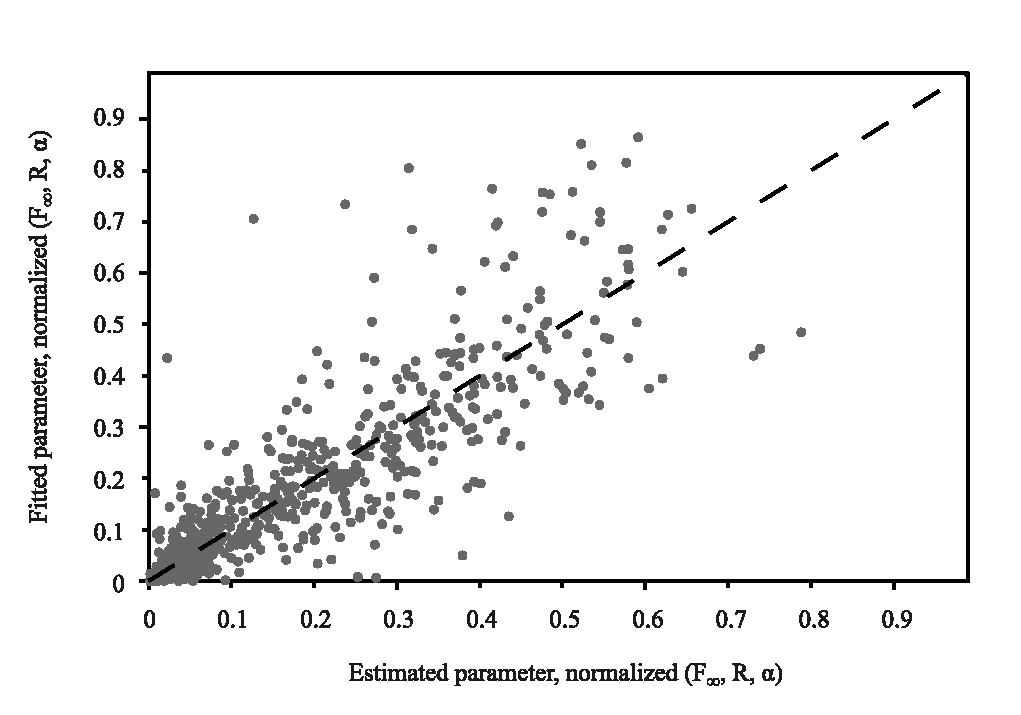
\includegraphics[width=\textwidth]{dpe_hyp.eps}
    \caption{Estimated regression parameters versus optimized regression 
    parameters (fitted after outliers were removed) for the hyperbolic model 
    (i.e., $F_{\infty}$, $R$, $\alpha$). Data is based on the monthly 
    partitioning of 25 flux towers during 2002. Parameter units have been 
    normalized for readability. The dashed line represents unity.}
    \label{fig:hmodest}
\end{figure}

Figure \ref{fig:hmodest} shows the relationship between the estimated parameters and optimized parameters for the hyperbolic model (i.e., equation \ref{eq:hypmod}).  
The units for each of three parameters have been normalized (i.e., values range between 0 and 1) for readability.  
The data is based on monthly regressions from 2002 of PPFD and NEE data pairs from 25 flux tower stations.  
A similar plot is shown in Figure \ref{fig:lmodest} where instead the regression parameters are shown for the linear model (i.e., equation \ref{eq:linmod}) for the same flux stations and time period.  
In both plots, the 1:1 line is shown for comparison.  
Both the hyperbolic and linear model parameter estimations exhibit moderately strong positively linear correlations to their optimized parameters ($r \approx 0.78$) suggesting that the dynamic parameterization methodology presented in equations \ref{eq:dpm1}--\ref{eq:dpm3} is suitable for this model.  
The simplicity of the dynamic parameterization model (requiring only mean, standard deviation, maximum and minimum of the observations) allows for the coefficients to be updated when new stations are included in the model.

%% ------------------------------------------------------------------------ %%
%% fig:lmodest | Linear model parameter estimates : optimized
%% ------------------------------------------------------------------------ %%
\begin{figure}[h!]
    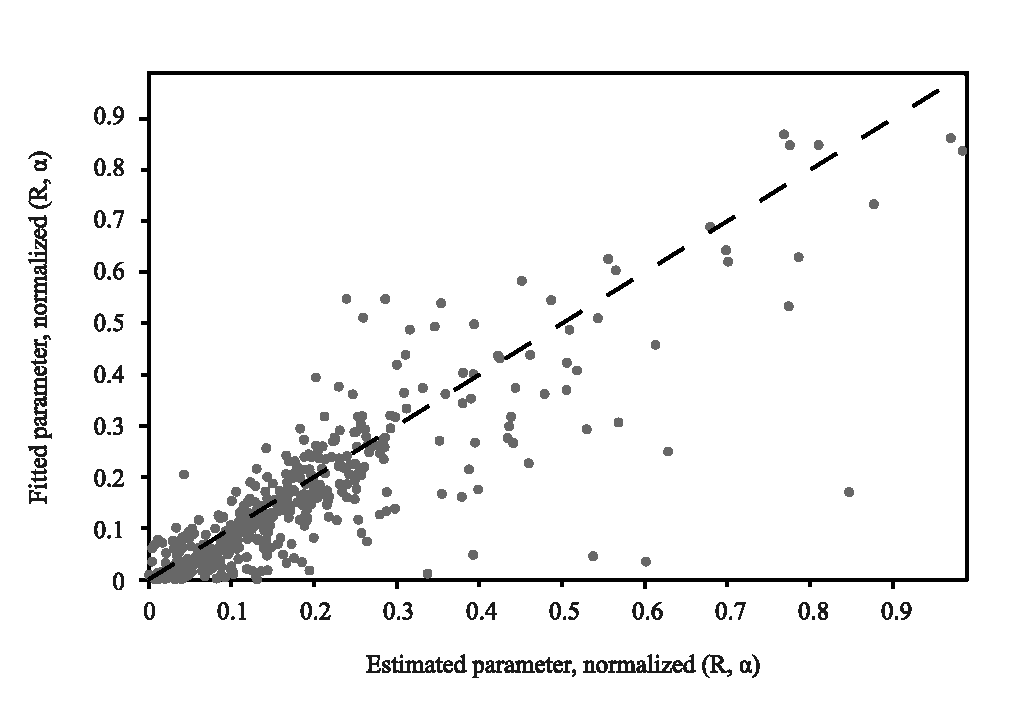
\includegraphics[width=\textwidth]{dpe_lin.eps}
    \caption{Estimated regression parameters versus optimized regression 
    parameters (fitted after outliers were removed) for the linear model 
    (i.e., $R$, $\alpha$). Data is based on the monthly partitioning of 25 flux 
    towers during 2002. Parameter units have been normalized for readability. 
    The dashed line represents unity.}
    \label{fig:lmodest}
\end{figure}

%% \\\\\\\\\\\\\\\\\\\\\\\\\\\\\\\\\\\\\\\\\\\\\\\\\\\\\\\\\\\\\\\\\\\\\\\\ %%
%% PART 3.5 -- CALCULATING GPP
%% //////////////////////////////////////////////////////////////////////// %%
\section{Calculating GPP}
\label{sec:calcgpp}
Following the regression of the flux partitioning parameters (i.e., $R$, $\alpha$, and $F_\infty$) from Eqns. \ref{eq:neemodels}, GPP can now be solved for:
%% ------------------------------------------------------------------------ %%
%% eq:gppmod | GPP models (Ruimy's models)
%% ------------------------------------------------------------------------ %%
\begin{subequations}
\label{eq:gppmod}
\begin{align}
    \text{GPP} &= \alpha\: Q \label{eq:gppl}\\
    \text{GPP} &= \frac{\alpha\: Q\: F_{\infty}}
                       {\alpha\: Q + F_{\infty}} \label{eq:gpph}
\end{align}
\end{subequations}
%% ------------------------------------------------------------------------ %%
%% fig:parti | Partitioning PPFD:NEE pairs
%% ------------------------------------------------------------------------ %%
\begin{figure}[h!]
    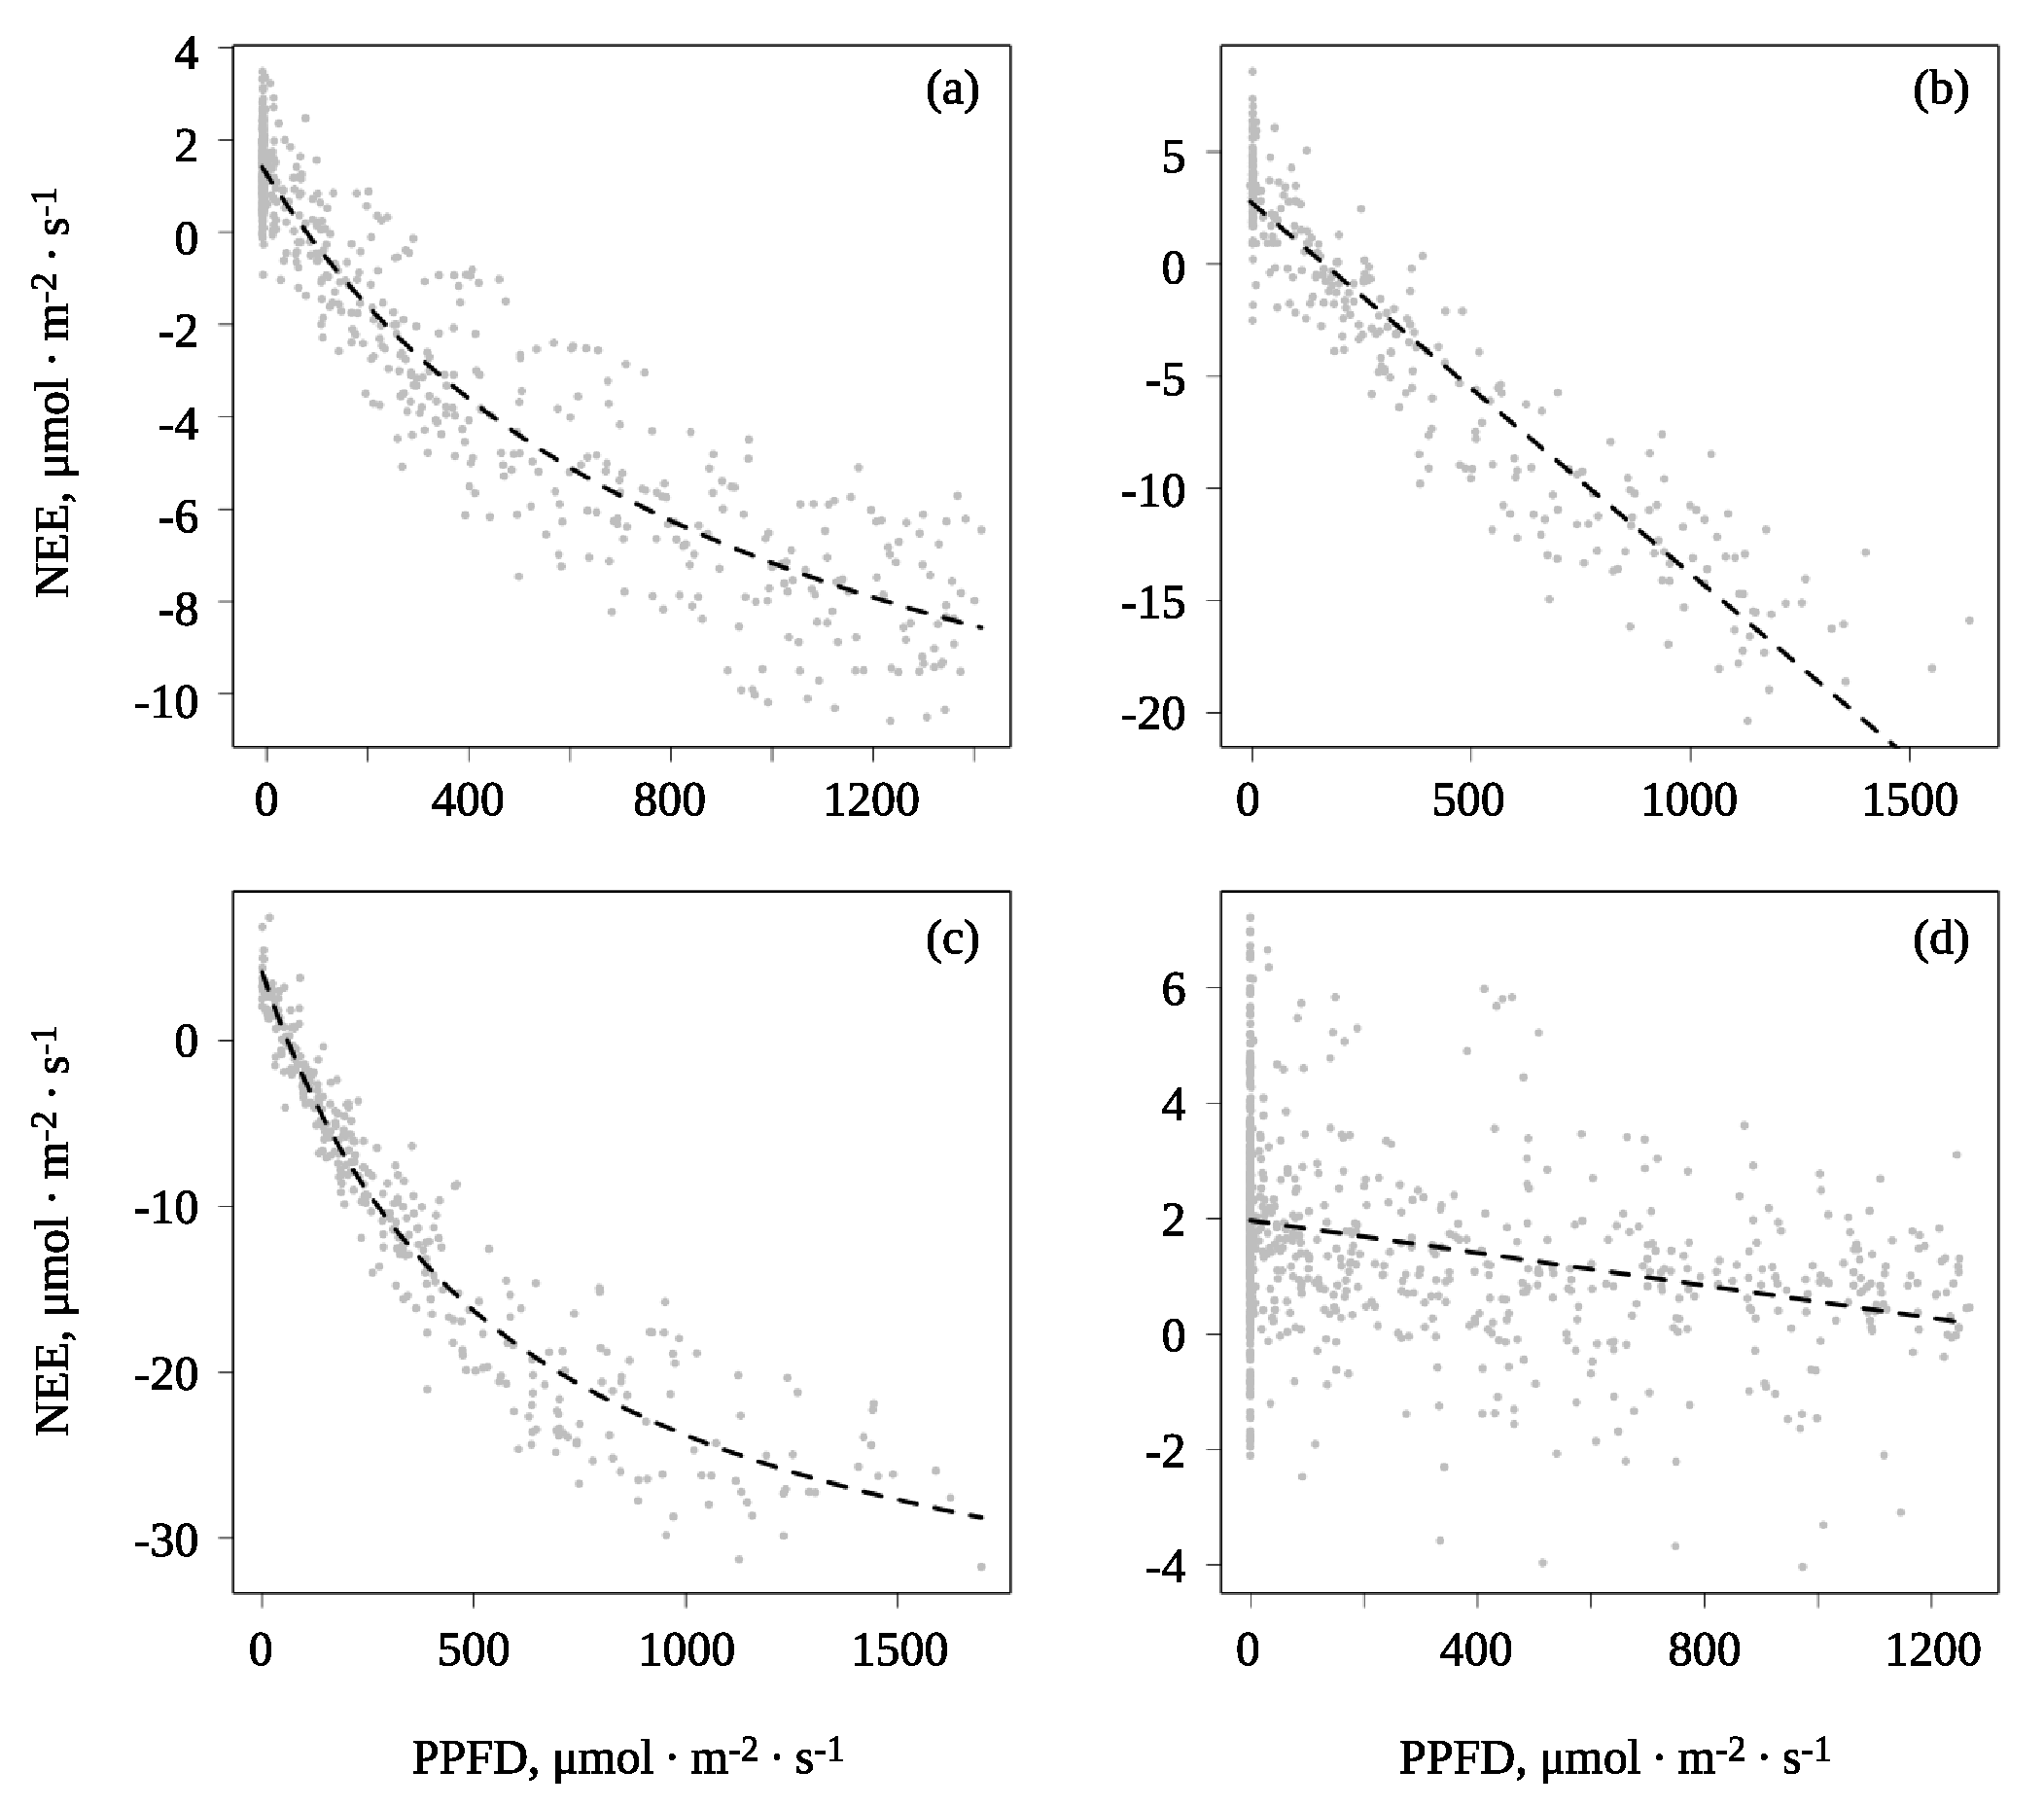
\includegraphics[width=\textwidth]{parti.eps}
    \caption{Flux partitioning of NEE and PPFD observations for stations (a) IL-
    Yat, Israel (Jan. 2002); (b) BE-Bra, Belgium (Aug. 2002); (c) DE-Hai, 
    Germany (Jul. 2002); (d) FR-Hes, France (Mar. 2002).  Data are fitted with 
    the rectangular hyperbola model in (a) and (c) and the linear model in (b) 
    and (d). }
    \label{fig:parti}
\end{figure}

Figure \ref{fig:parti} presents example months of flux partitioning from four flux towers.  
In Figs. \ref{fig:parti}a and \ref{fig:parti}c, the trend between NEE and PPFD observations suits the hyperbolic model (i.e., equation \ref{eq:hypmod}), $R^{2}$ is 0.91 and 0.93, respectively. 
On the contrary, the trend presented in Fig. \ref{fig:parti}b cannot be clearly distinguished as linear from hyperbolic as both models perform equally well ($R^{2}$ is 0.90 and 0.91 for the linear and hyperbolic fits, respectively). 
The high level of variability in Fig. \ref{fig:parti}d results in poor regression fitting and is therefore difficult to distinguish between hyperbolic and linear model fits ($R^{2}\approx$0.1 for both linear and hyperbolic model fits).

%%
%% Add error propagation
%%
%% \\\\\\\\\\\\\\\\\\\\\\\\\\\\\\\\\\\\\\\\\\\\\\\\\\\\\\\\\\\\\\\\\\\\\\\\ %%
%% PART 3.5.1 -- ERROR PROPAGATION
%% //////////////////////////////////////////////////////////////////////// %%
\subsection{Error propagation}
\label{sec:mst1errprop}
During the flux partitioning of NEE and PPFD observations, the fitting parameters used to calculate GPP (i.e., Eq. \ref{eq:gppl} and Eq. \ref{eq:gpph}) are estimated.  
The parameter estimates include some uncertainty or associated error.  
To account for these errors in the calculation of GPP, a methodology of arithmetic error propagation is employed \parencite{caldwell14}.  
The general formula for the error propagation where $Y=f(A,B,C)$ is given as \parencite{ku66}:
%% ------------------------------------------------------------------------ %%
%% eq:errprop | Propagation of Error
%% ------------------------------------------------------------------------ %%
\begin{equation}
\label{eq:errprop}
	s_{y} = \sqrt{
		\left(\frac{\partial Y}{\partial A}\right)^{2}\; s_{a}^{2} +
		\left(\frac{\partial Y}{\partial B}\right)^{2}\; s_{b}^{2} +
		\left(\frac{\partial Y}{\partial C}\right)^{2}\; s_{c}^{2}
		}
\end{equation}

\noindent where $s$ is the standard deviation (i.e., error).\\

For the rectangular hyperbola formula for GPP (i.e., Eq. \ref{eq:gpph}), let $A = \alpha$, $B = F_{\infty}$, and $C = \text{PPFD}$ such that:
%% ------------------------------------------------------------------------ %%
%% eq:hpartial | Partial derivatives for error propagation:
%% ------------------------------------------------------------------------ %%
\begin{subequations}
\label{eq:hpartial}
\begin{align}
    \frac{\partial Y}{\partial A}&= \frac{F_{\infty}\: \text{PPFD}\: 
                                    \left( \alpha\: \text{PPFD} + F_{\infty} 
                                    \right) - \alpha\: F_{\infty}\: 
                                    \text{PPFD}^{2}}{\left(\alpha\: 
                                    \text{PPFD} + F_{\infty} \right)^{2}} 
                                    \label{eq:hparta}\\
    \frac{\partial Y}{\partial B}&= \frac{\alpha\: \text{PPFD}\: 
                                    \left( \alpha\: \text{PPFD} + F_{\infty} 
                                    \right) - \alpha\: F_{\infty}\: 
                                    \text{PPFD}}{\left(\alpha\: 
                                    \text{PPFD} + F_{\infty} \right)^{2}} 
                                    \label{eq:hpartb}\\
    \frac{\partial Y}{\partial C}&= \frac{\alpha\: F_{\infty}\: 
                                    \left( \alpha\: \text{PPFD} + F_{\infty} 
                                    \right) - \alpha^{2}\: F_{\infty}\: 
                                    \text{PPFD}}{\left(\alpha\: 
                                    \text{PPFD} + F_{\infty} \right)^{2}}  
                                    \label{eq:hpartc}
\end{align}
\end{subequations}

By substituting Eqs. \ref{eq:hparta}--\ref{eq:hpartc} into Eq. \ref{eq:errprop} and assigning the corresponding error values to $s_{a}$, $s_{b}$, and $s_{c}$ (note: the measurement of PPFD is assumed to be error-free, $s_{c} = 0$) the associated error for GPP can be calculated. 

In the more trivial case of the linear equation for GPP (i.e., Eq. \ref{eq:gppl}), the error propagation is directly proportional to the coefficient $alpha$ and its associated error.
